% ===========================================================================
% Modello di tesi di laurea triennale
% Dipartimento di Ingegneria, Università degli Studi di Messina
% Relatore: Chiar.mo Prof. Francesco Longo
%
% COME SI USA SU OVERLEAF
%   1. Su overleaf.com: New Project > Upload Project > scegliere lo .zip
%      scaricato dal sito
%   2. Menu > Compiler: pdfLaTeX  (è già il valore predefinito)
%   3. Riempire i campi qui sotto e premere Recompile
%
% La bibliografia usa BibTeX: le voci si scrivono in bibliografia.bib e
% Overleaf lancia bibtex da sé. In locale servono due compilazioni:
%   pdflatex tesi && bibtex tesi && pdflatex tesi && pdflatex tesi
%
% Il testo in corsivo grigio dentro i capitoli è una guida: va cancellato
% mano a mano che si scrive.
% ===========================================================================

\documentclass[12pt,a4paper,oneside]{report}

\usepackage[T1]{fontenc}
\usepackage{mathptmx}   % Times, come nei modelli Word
\usepackage[utf8]{inputenc}
\usepackage[italian]{babel}
\usepackage[a4paper,margin=3cm]{geometry}
\usepackage{graphicx}
\usepackage{float}   % [H]: figure e tabelle restano dove sono scritte
\usepackage{array}
\usepackage{setspace}
\usepackage{booktabs}
\usepackage{caption}
\usepackage{listings}
\renewcommand{\lstlistingname}{Listato}
\usepackage{xcolor}
\usepackage[hidelinks]{hyperref}

\usepackage{remreset}
\makeatletter   % figure, tabelle e snippet numerati di seguito, non per capitolo
\@removefromreset{figure}{chapter}
\@removefromreset{table}{chapter}
\makeatother
\renewcommand{\thefigure}{\arabic{figure}}
\renewcommand{\thetable}{\arabic{table}}

\setlength{\parindent}{0pt}
\setlength{\parskip}{6pt}

\newcommand{\guidabib}{\guida{I riferimenti si elencano nell'ordine in cui compaiono nel testo e si numerano: il numero è quello con cui li hai citati fra parentesi quadre, e di questo si occupa BibTeX da solo. Lo stile è IEEE, quello degli esempi che seguono — un articolo, un libro e una pagina web — e lo applica \texttt{ieeetr}, impostato in \texttt{tesi.tex}. Per raccogliere i dati il modo più rapido è il pulsante «Cita» di Google Scholar: ignora gli stili che propone e prendi il collegamento BibTeX in fondo al riquadro, da incollare in \texttt{bibliografia.bib}.}}
\makeatletter   % la bibliografia porta con se` titolo, voce d'indice e guida
\renewenvironment{thebibliography}[1]
  {\chapter*{\bibname}\addcontentsline{toc}{chapter}{\bibname}%
   \guidabib
   \list{\@biblabel{\@arabic\c@enumiv}}%
        {\settowidth\labelwidth{\@biblabel{#1}}%
         \leftmargin\labelwidth \advance\leftmargin\labelsep
         \@openbib@code \usecounter{enumiv}\let\p@enumiv\@empty
         \renewcommand\theenumiv{\@arabic\c@enumiv}}%
   \sloppy \clubpenalty4000 \@clubpenalty\clubpenalty
   \widowpenalty4000 \sfcode`\.\@m}
  {\def\@noitemerr{\@latex@warning{Bibliografia vuota}}\endlist}
\makeatother

\onehalfspacing
\newcolumntype{R}[1]{>{\raggedleft\arraybackslash}p{#1}}
\newcommand{\guida}[1]{{\itshape\color{gray}#1\par}}
\newcommand{\sugg}[1]{\nopagebreak\par\vspace{2pt}%
  {\normalfont\itshape\normalsize\color{gray}#1}}
\newcommand{\esempio}[1]{#1\par}
\setcounter{secnumdepth}{3}   % numera anche le sotto-sottosezioni
\setcounter{tocdepth}{3}      % e le mostra nell'indice

\lstset{
  numberbychapter=false,
  numbers=left, numberstyle=\tiny\color{gray}, numbersep=8pt,
  basicstyle=\ttfamily\small, keywordstyle=\color{blue!60!black},
  commentstyle=\color{gray}, stringstyle=\color{green!40!black},
  frame=single, rulecolor=\color{gray!40},
  breaklines=true, showstringspaces=false, captionpos=b
}

% --- DA RIEMPIRE -----------------------------------------------------------
\newcommand{\corsodilaurea}{Corso di Laurea in \dotfill}
\newcommand{\titolotesi}{Titolo della tesi}
\newcommand{\candidato}{Nome Cognome}
\newcommand{\relatore}{Chiar.mo Prof. Francesco Longo}
\newcommand{\annoaccademico}{20\ldots/20\ldots}
% ---------------------------------------------------------------------------

\begin{document}

% ---------------------------------------------------------------------------
% Frontespizio. Compilarlo da solo serve per stamparlo e farlo firmare: il PDF
% firmato e` uno dei file da caricare su Esse3 con la domanda di laurea.
% Dentro la tesi non si compila da solo, viene incluso da tesi.tex.
% ---------------------------------------------------------------------------
\begin{titlepage}
  \centering

  
\includegraphics[width=3.2cm]{logo-unime.png}\\[0.7cm]
  {\Large\bfseries UNIVERSIT\`A DEGLI STUDI DI MESSINA}\\[0.25cm]
  {\large DIPARTIMENTO DI INGEGNERIA}\\[0.35cm]
  {\large\bfseries \corsodilaurea}\\[0.12cm]
  \rule{\textwidth}{0.4pt}

  \vfill
  {\LARGE\bfseries \titolotesi}
  \vfill

  \begin{tabular}{@{}p{0.47\textwidth}@{\hfill}R{0.47\textwidth}@{}}
    Relatore:                & Tesi di Laurea di:        \tabularnewline[0.15cm]
    \textbf{\relatore}       & \textbf{\candidato}       \tabularnewline
  \end{tabular}

  \vspace{1.6cm}
  \rule{\textwidth}{0.4pt}\\[0.15cm]
  {\bfseries ANNO ACCADEMICO \annoaccademico}

\end{titlepage}


\tableofcontents
\listoffigures
\listoftables

\chapter*{Abstract}
\addcontentsline{toc}{chapter}{Abstract}
\guida{Nota valida per tutta la tesi: puoi usare gli strumenti di intelligenza artificiale per migliorare la forma, la chiarezza e la correttezza della lingua, non per generare contenuti, risultati o argomentazioni che non sapresti spiegare e difendere.}
\guida{Nota valida per tutta la tesi: elimina tutti i suggerimenti in grigio
nella versione finale della tua tesi.}
\guida{L'abstract deve essere lungo una pagina e descrivere brevemente il problema, che cosa è stato fatto e il risultato principale. Si scrive per ultimo, quando si sa che cosa si è ottenuto.}

\chapter{Introduzione}
\guida{Ogni capitolo si apre con un paragrafo che ne annuncia il contenuto,
fuori da qualunque sezione. Per esempio:}
\esempio{In questo capitolo si introduce il contesto in cui il lavoro si
colloca, si enuncia l'obiettivo della tesi e si descrive l'organizzazione dei
capitoli che seguono.}

\section{Il contesto}
\guida{Di cosa si parla in questa tesi e perché il problema esiste. Scrivilo pensando a qualcuno
che conosce l'informatica ma non è esperto dell'argomento della tua tesi.}

\section{Obiettivo della tesi}
\guida{Che cosa ti sei proposto di fare. E soprattutto qual è il tuo
contributo, cioè che cosa c'era prima e che cosa c'è adesso grazie al tuo
lavoro. È la prima cosa che una commissione cerca ed è quella che gli studenti
dimenticano più spesso.}

\section{Struttura della tesi}
\guida{La mappa: un paragrafo che dice cosa si trova in ciascun capitolo, così
chi legge sa dove andare.}

\chapter[Background]{Background \sugg{(modifica il titolo come ti piace di più)}}
\guida{Uno o più capitoli. Il criterio per decidere cosa mettere in questi capitoli è questo: immagina che un collega debba continuare il tuo lavoro e debba leggere la tua tesi per farlo. Che cosa deve conoscere e studiare per capire a fondo quello che hai fatto e come proseguirlo? Ecco quello che va in questi capitoli.}
\esempio{In questo capitolo si richiamano le nozioni necessarie a seguire il resto del lavoro: la tecnologia X, il protocollo Y e le tecniche con cui in letteratura si affronta il problema Z.}
\guida{Ogni capitolo può essere organizzato in più sezioni, con più sottosezioni e sotto-sottosezioni ciascuna.}

\section{Titolo della prima sezione}
\guida{Anche le sezioni si aprono annunciando il proprio contenuto, con una frase sola. Per esempio:}
\esempio{Questa sezione descrive la tecnologia X, a partire dal modello di esecuzione per arrivare ai limiti che ne derivano.}
\guida{Questo è anche il capitolo in cui compaiono quasi tutte le fonti. Si citano con il numero fra parentesi quadre, a fine periodo prima del punto. Un possibile esempio è il seguente:}
\esempio{La migrazione di container nel fog computing è stata studiata confrontando le tecniche cold, pre-copy e post-copy~\cite{esempio-articolo}. Una trattazione sistematica degli algoritmi impiegati si trova in~\cite{esempio-libro}, mentre la documentazione ufficiale del runtime descrive l'interfaccia utilizzata~\cite{esempio-web}.}
\subsection{Titolo della sottosezione}
\guida{Si scende di livello quando una sezione contiene due o più argomenti che meritano un titolo proprio. Se ce n'è uno solo, la sottosezione non serve.}

\subsubsection{Titolo della sotto-sottosezione}
\guida{Terzo e ultimo livello. Più in basso di così la numerazione diventa illeggibile: se serve, conviene ripensare l'organizzazione del capitolo.}

\section{Titolo della seconda sezione}

\subsection{Titolo della sottosezione}

\subsubsection{Titolo della sotto-sottosezione}

\chapter[Il lavoro svolto]{Il lavoro svolto \sugg{(modifica il titolo come reputi più descrittivo del tuo lavoro specifico)}}
\guida{Uno o più capitoli, il cuore della tesi. Spiega il tuo lavoro nel dettaglio: l'architettura del sistema, del software o dell'algoritmo su cui hai lavorato, e le scelte che hai fatto con le loro ragioni.}
\esempio{In questo capitolo si presenta l'architettura del sistema realizzato, se ne discutono le scelte implementative e si riportano le misure sperimentali raccolte.}
\guida{Ogni capitolo può essere organizzato in più sezioni, con più sottosezioni e sotto-sottosezioni ciascuna.}

\section{Architettura del sistema}
\guida{Metti molte figure: pensa fin d'ora a come farai la presentazione il giorno della laurea, e disegna quello che spiegherai a voce. Per l'architettura e il comportamento sono utili i diagrammi UML più comuni, activity diagram, sequence diagram, class diagram.}

\guida{Ogni figura va richiamata nel testo: una figura che non viene mai citata è decorazione. La didascalia sta sotto la figura. Un possibile esempio è il seguente:}
\esempio{L'architettura complessiva del sistema è rappresentata in Figura~\ref{fig:esempio}.}

\begin{figure}[H]
  \centering
  
\includegraphics[width=4cm]{logo-unime.png}
  \caption{Didascalia della figura.}
  \label{fig:esempio}
\end{figure}

\section{Sviluppo software}
\guida{Inserisci solo i listati significativi e spiegane le parti che contano, quelle in cui si vede una scelta implementativa. Non incollare lunghe porzioni di codice: scegli quelle che aiutano a capire il lavoro svolto.}

\guida{Anche i listati vanno richiamati nel testo: un listato che non viene mai citato è decorazione. La didascalia sta sotto il listato. Un possibile esempio è il seguente:}
\esempio{La funzione che calcola la somma è riportata nel Listato~\ref{lst:esempio}.}

\begin{lstlisting}[language=C,caption={Didascalia del listato.},label=lst:esempio]
int somma(int a, int b) {
    return a + b;
}
\end{lstlisting}

\section{Misure e risultati}
\guida{Riporta tutte le misure sperimentali che sei riuscito a fare e le osservazioni che se ne possono trarre sull'efficienza e sulle prestazioni.}
\guida{Quando i risultati vengono da misure ripetibili, fai un numero adeguato di repliche e riporta anche la variabilità, per esempio la deviazione standard o gli intervalli di confidenza. Una media senza un'indicazione della variabilità non dice quanto ci si possa fidare del confronto.}

\guida{Anche le tabelle vanno richiamate nel testo: una tabella che non viene mai citata è decorazione. La didascalia sta sopra la tabella. Un possibile esempio è il seguente:}
\esempio{I tempi misurati nelle due configurazioni sono riportati in Tabella~\ref{tab:esempio}.}

\begin{table}[H]
  \centering
  \caption{Didascalia della tabella.}
  \label{tab:esempio}
  \begin{tabular}{lrr}
    \toprule
    Configurazione & Tempo medio (ms) & Deviazione standard \\
    \midrule
    A & 12,4 & 0,8 \\
    B & 31,7 & 2,1 \\
    \bottomrule
  \end{tabular}
\end{table}

\guida{Un grafico è una figura a tutti gli effetti, quindi anche lui va richiamato nel testo e ha la didascalia sotto. Un possibile esempio è il seguente:}
\esempio{L'andamento del tempo di risposta al crescere del carico è riportato in Figura~\ref{fig:grafico}, dove le barre verticali sono gli intervalli di confidenza al 95\%.}

\begin{figure}[H]
  \centering
  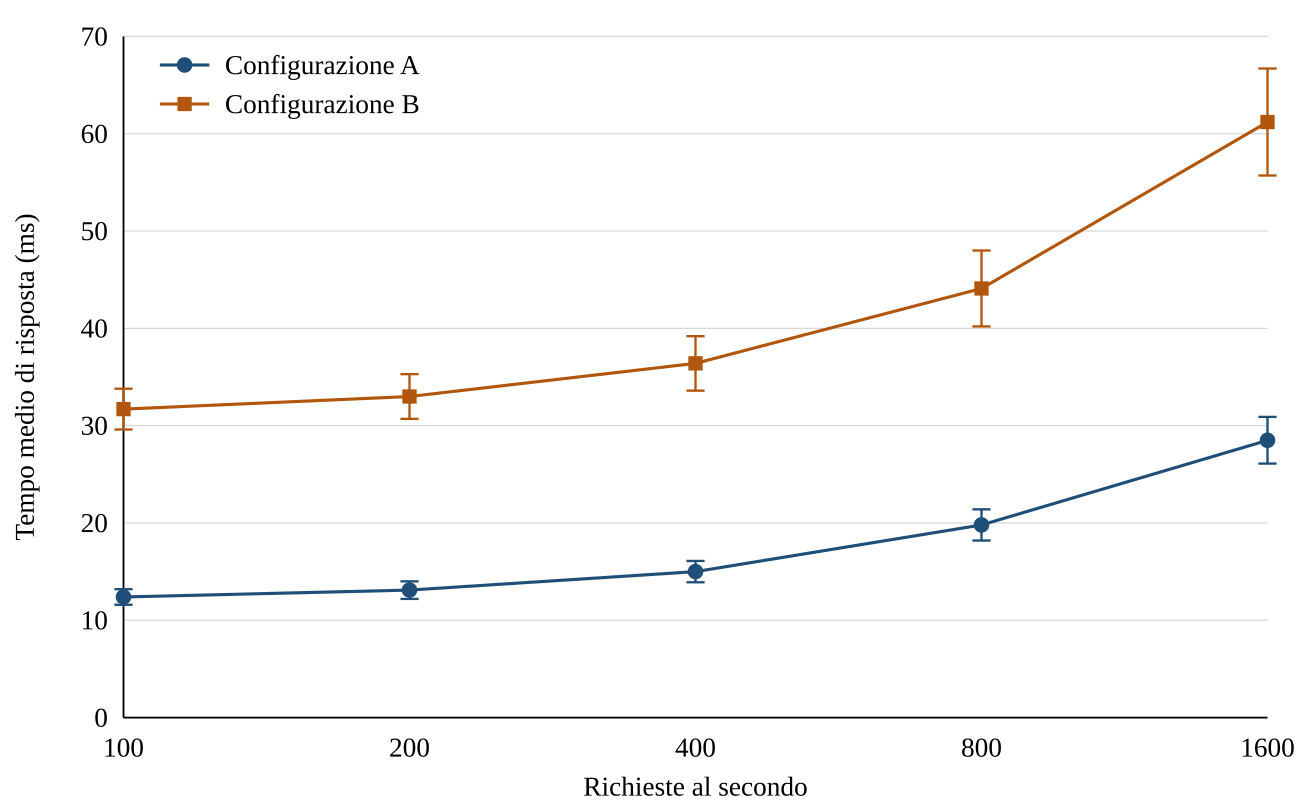
\includegraphics[width=11cm]{grafico.png}
  \caption{Tempo medio di risposta al crescere del carico, con intervalli di confidenza al 95\%.}
  \label{fig:grafico}
\end{figure}

\chapter{Conclusioni}
\guida{Anche l'ultimo capitolo si apre annunciando il proprio contenuto.}
\esempio{In questo capitolo si riassumono i risultati ottenuti, se ne
discutono i limiti e si indicano le direzioni in cui il lavoro può proseguire.}
\guida{Le conclusioni non introducono nuovi risultati né nuove informazioni tecniche: interpretano e sintetizzano quello che i capitoli precedenti hanno già presentato. Riassumi brevemente i risultati ottenuti. Dichiara anche i limiti del lavoro: una tesi che li riconosce è più credibile, non meno. Chiudi con i possibili sviluppi futuri, cioè da dove ripartirebbe quel collega.}

\bibliographystyle{ieeetr}
\bibliography{bibliografia}

\end{document}
